\entry{Semanas del 24/11/2025} 
\section{Martes 25/11/2025} 
Analicé las señales de las mediciones de la semana pasada para estimar los parámetros de calibración de los sensores y después analicé y calibré las distintas series temporales con los distintos forzados.  


Los puntos durante el llenado de la cuba son los siguientes:

\begin{figure}[th!]
	\centering
	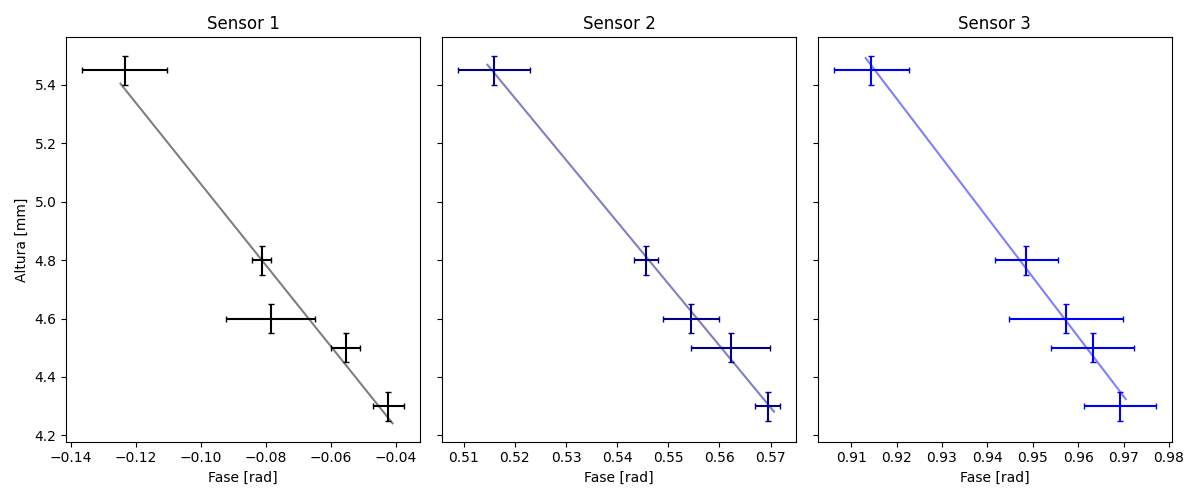
\includegraphics[width=0.87\linewidth]{Figures/20_11_2025/Datos_calibracion_tres_sensores_bien}
	\caption{Puntos para la calibración simultáneo de los tres sensores al ir llenando la curva. IMPORTANTE: las unidades deberían ser cm en lugar de mm.}
	\label{fig:datoscalibraciontressensoresbien}
\end{figure}

El sensor 1 es el más largo (y más cercano al toroide), y así en orden hasta el más corto. Los parámetros de calibración son: 

\begin{figure}[th!]
	\centering
	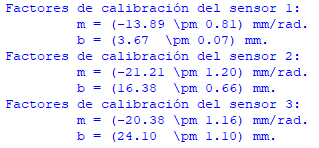
\includegraphics[width=0.7\linewidth]{Figures/20_11_2025/Datos_calibracion_tres_sensores_bien_parámetros}
	\caption{Parámetros de calibración de los tres sensores. IMPORTANTE: las unidades deberían ser cm en lugar de mm.}
	\label{fig:datoscalibraciontressensoresbienparametros}
\end{figure} 



